% !TeX root = ../index.tex

\section{Reactive \acrlongpl{is}}\label{sec:reactive-is}

\citeauthor{boner_reactive_2014} describe how modern \glspl{is} of different domains all exhibit similar qualities.
\citetitle{boner_reactive_2014} summarizes those qualities and dubs the systems which feature them \enquote{reactive} \parencite{boner_reactive_2014}.
Figure \ref{fig:reactive-traits} shows the qualities of a reactive system and their relation to each other.
% Put into the context of the quality dimensions defined by the \citetitle{iso_25010_2011} standard,
% the reactive qualities cover only \enquote{Performance Efficiency} and \enquote{Reliability}.
% While the other quality dimensions of the \citeauthor{iso_25010_2011} standard are certainly also important, this work focuses on the two mentioned before.\todo{improve sentence flow}

\begin{figure}[H]
  \centering
  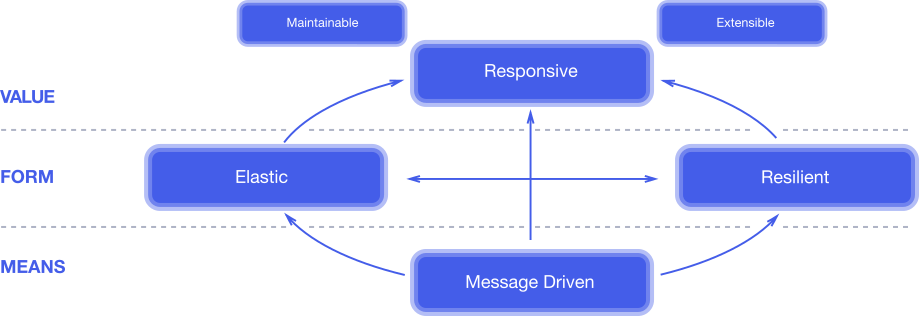
\includegraphics[width=\linewidth]{reactive-traits.png}
  \caption{The Qualities of a Reactive System \parencite{boner_reactive_2014}}
  \label{fig:reactive-traits}
\end{figure}

According to \cite{boner_reactive_2014}, reactive systems are \emph{responsive}, meaning that they have low upper ceilings for their response times and meet them consistently.
Furthermore, reactive systems are \emph{resilient}.
They remain responsive in the face of failure.
Furthermore, a system needs to remain responsive under varying work-load.
It needs to be \emph{elastic}, to be reactive.
The fourth quality, message-driven, is examined more closely in section \ref{sec:mom}

All of these qualities cover the technological perspective on reactive systems.
However, there is a business perspective to the term, too.
Reactive systems also need to be flexible.
They need be able to to respond and change quickly according to changing requirements.
For example due to changing customer or market needs.
\citeauthor{beck2001agile} describe this quality as part of their \citetitle{beck2001agile} \parencite{beck2001agile}.
The text will refer to this quality as \emph{flexibility} from here on.

Different design and work patterns have emerged to create reactive systems.
The following section explores an increasingly popular one: microservice architecture \parencite{loukides_microservice_adoption_2020}.

\subsection{Microservice Architecture}

\citeauthor{richardson_microservices_2019} defines the microservice pattern as \enquote{an architectural style that functionally decomposes an application into a set of services} \parencite[11]{richardson_microservices_2019}.
The services are supposed to be loosely coupled, independently deployable, and scalable.
They are also small enough to be developed by a single, largely autonomous team.
The compartmentalization of the application allows it to tolerate partial failure, meaning that if a single service fails, the rest of the application may stay partially functional.
\parencite[14f.]{richardson_microservices_2019}
These qualities contribute to the application's overall elasticity, resilience, and flexibility.

It is pointed out by \citeauthor{fowler_microservices_2014} that microservices commonly integrate with each other via synchronous communication protocols like \glspl{rpc} or HTTP \parencite{fowler_microservices_2014}.
This introduces different forms of coupling to the system.
First, the services need to know routes via which they can reach another directly.
Second, the services need to know not only the structure of the data they exchange but also each others' \glspl{api}.
Third, the synchronous nature of the communication couples the services in the dimension of time.
A service either completes a request in time, or the request reaches a timeout and fails.
It is for this reason that many architectures rely on asynchronous, message-driven communication via \gls{mom} \parencite{fowler_microservices_2014}.

\subsection{\acrlong{mom}}\label{sec:mom}

The fourth quality of reactive systems defined by \cite{boner_reactive_2014} is \emph{message-driven}.
Message-driven systems \enquote{rely on asynchronous message-passing to
establish a boundary between components that ensures loose coupling, isolation,
location transparency, and provides the means to delegate errors as messages.} \parencite{boner_reactive_2014}
As shown in figure \ref{fig:reactive-traits}, the message-driven quality forms the foundation for achieving all other qualities of a reactive system.

\cite{banavar_case_1999} coined the term of \acrlong{mom} for dedicated software components meant to integrate disparate applications in a distributed system by facilitating asynchronous message-passing.
It is based in part on the publish/subscribe semantics described in \cite{oki_information_1993} which are still present in the more comprehensive exploration of \gls{mom} in \cite{curry_message-oriented_2004} and prevail to this day.

There exist multiple established protocols which implement the patterns of \gls{mom} like AMQP and MQTT\footcites{amqp}{mqtt} and software solutions implementing the protocols (also called message brokers) like RabbitMQ or Mosquitto\footcites{rabbitmq}{mosquitto}.
While implementation details and terminology vary between protocols and brokers, the general patterns stay the same.

Clients \emph{publish} packets of data called \emph{messages} to a logical communication channel managed by the broker.
From here on, the text refers to such communication channels as \emph{topics}.
Clients can also \emph{subscribe} themselves to these topics and receive messages published to them.
Message delivery may be transient or persistent, meaning that messages are either delivered immediately to the subscribers of a topic by the broker or that the broker stores the messages in subscriber-specific, first-in-first-out queues.
Queues allow subscribers to consume messages at their own pace and become temporarily unavailable without losing messages.
\parencite{curry_message-oriented_2004}

However, one popular message broker does things a little differently.
The following section examines the ways in which Apache Kafka implements the patterns of \gls{mom}.

\subsection{Apache Kafka}

The LinkedIn employees \citeauthor{kreps_kafka_2011} introduced their new \enquote{Event Streaming Platform} \emph{Kafka} in \citeyear{kreps_kafka_2011} \parencite{kreps_kafka_2011}.
Over a decade later, the project has since joined the Apache foundation and \enquote{[m]ore than 80\% of all Fortune 100 companies trust, and use [it.]} \parencite{apache_software_foundation_apache_nodate}.

\citeauthor{kreps_kafka_2011} describe Kafka as \enquote{[\ldots] a novel messaging system for log processing [\ldots] that combines the benefits of traditional log aggregators and messaging systems.} \parencite{kreps_kafka_2011}.
Similar to traditional \gls{mom}, \emph{producers} publish messages to logical communication channels called topics and \emph{consumers} can subscribe to topics to consume messages.
In contrast to traditional \gls{mom} however, topics are backed by one or more \emph{partitions}, an append-only data structure stored on the hard drive of a server running Kafka called a \emph{broker}.
Therefore, Kafka persists all messages sequentially for a configurable time even if the brokers restart.
Producers address messages to a topic but actually always publish them to a partition.
To which partition they publish a message if there are multiple is determined by a partitioning algorithm.
Partitions can also have replicas on other brokers, making Kafka tolerant against the failure of single servers.
\parencite{kreps_kafka_2011}

A message in Kafka does not have a dedicated identifier.
Instead, a message's logical offset within its partition identifies it.
Consumers consume messages sequentially and move a pointer to the next offset after they have processed the message at the current position.
Furthermore, consumers can form groups in which no two members subscribe to the same partition, thereby achieving a simple load balancing mechanism.
That also makes the number of partitions that a topic has the maximum degree of parallelism with which consumers can consume its messages.
\parencite{kreps_kafka_2011}

Kafka is not only useful for processing the kinds of log data that are proposed in \cite{kreps_kafka_2011}: activity (e.~g. user logins, clicks, \enquote{likes}, \ldots) and operational data (e.~g. \gls{cpu} or disk utilization, HTTP requests, \ldots).
\cite{stopford_designing_2018}, for example, outlines how Kafka can serve as the basis of a business application's entire state management and internal communication.
The design implements concepts from the \gls{ddd} community like Event Sourcing \parencite{fowler_event_sourcing_2005} and \gls{cqrs} \parencite{fowler_cqrs_2011} with Kafka's log-based messaging at the center.
The potential use cases of Kafka are therefore plentiful.
